\chapter{Overview Distribuit}
\label{sec:overview_distribuita}

Infrastructura este implementată într-o rețea virtualizată (containere Docker) și este compusă din 4 servere de baze de date (noduri):

Serverul 1 (SV1) - Modulul B2C: Gestionează operațiunile și datele aferente clienților de tip persoană fizică. Aici sunt stocate fragmentele orizontale primare și derivate pentru clienții și tichetele fizice.

Serverul 2 (SV2) - Modulul B2B: Gestionează operațiunile și datele aferente clienților de tip persoană juridică (companii). Aici sunt stocate fragmentele orizontale primare și derivate pentru clienții și tichetele juridice.

Serverul 3 (SV3) - Modulul de Securitate: Nod izolat, dedicat exclusiv stocării datelor sensibile de autentificare ale agenților (adrese de email și hash-uri pentru parole), rezultate în urma fragmentării verticale a relației Agent.

Serverul 4 (SV4) - Master Data (Nod Central): Stochează nomenclatoarele, dicționarele globale (statusuri, priorități, categorii, departamente) și KB (Knowledge Base). Pentru a optimiza traficul de rețea, aceste date sunt replicate către SV1 și SV2 prin intermediul Mat. Views.

Serverul 1 este hostat pe un VPS separat in container docker - IP 10.80.0.40 - p1521

Serverul 2 este hostat pe un VPS separat in container docker - IP 10.80.0.41 - p1521

Serverul 3 si Serverul 4 sunt hostate pe Homelab separate in containere docker - IP 10.80.0.30 - SV3 p1521 | SV4 p1522

Mai jos este o diagrama a distirbuitii:
\begin{figure}[H]
    \centering
    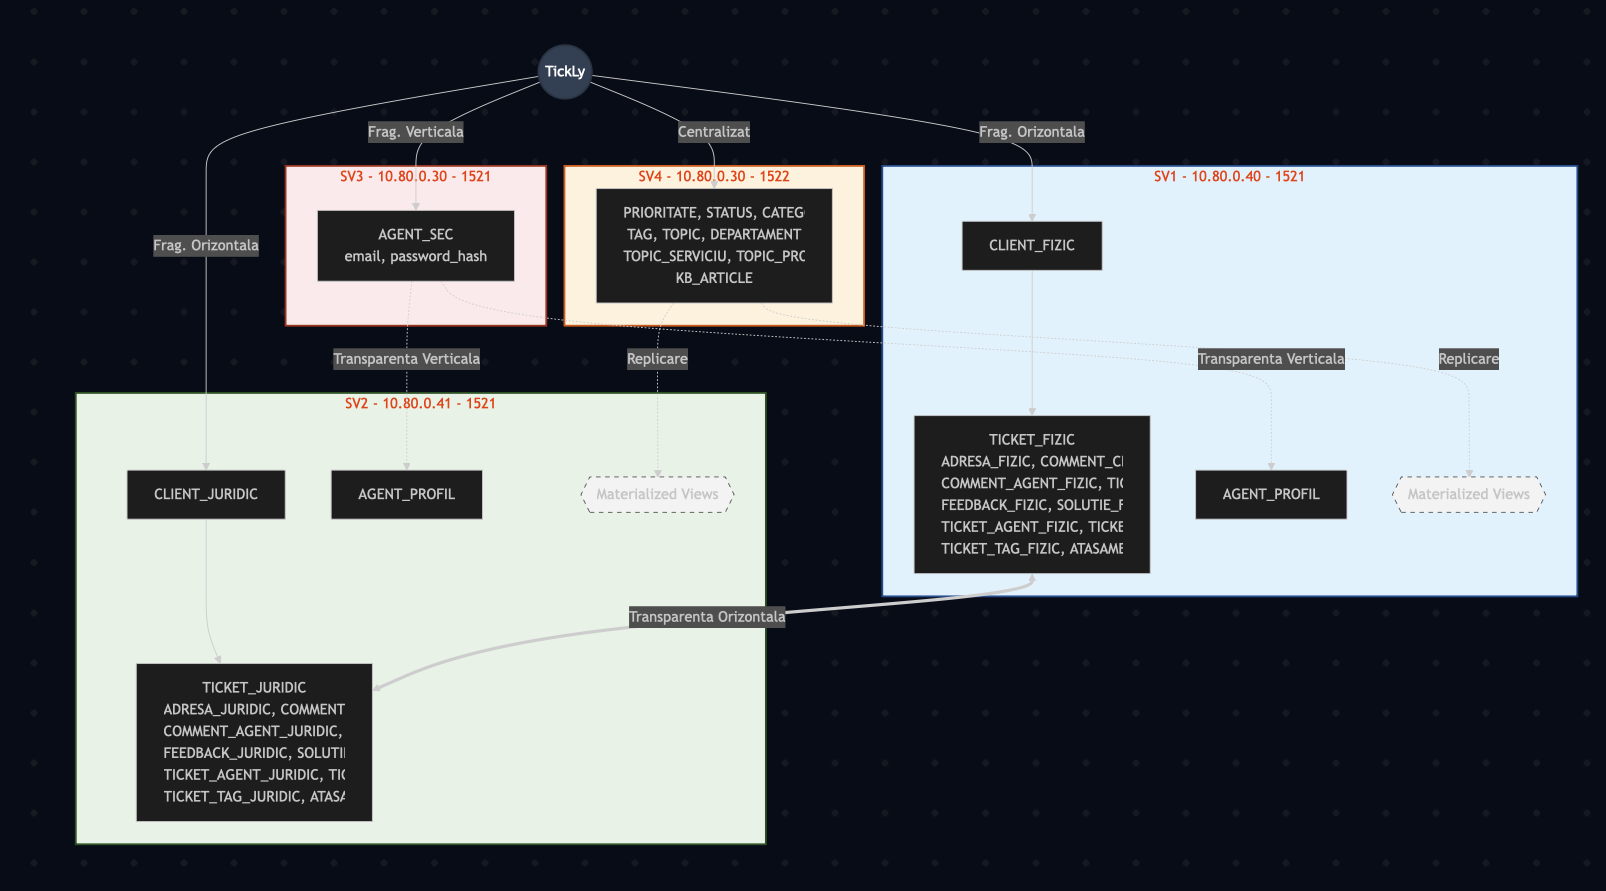
\includegraphics[width=1.0\textwidth]{./assets/replicare/diagrama.png}
    \caption{Diagrama Distribuirii}
    \label{fig:distribution_diagram}
\end{figure}